
% asset_id: FAS1VectorsTikZ-001
% asset_type: tikz
% topic_id: FAS1Vectors
% unit_code: FAS1
% topic_code: FAS1-VEC
% related_lesson_file: FAS1_vectors_lesson.md
% related_lesson_section: # 9. Visual Asset Integration
% source: FP1-Chp1-Vectors.pdf + transcripts.md where relevant
\documentclass[tikz,border=8pt]{standalone}
\usepackage{amsmath}
\usepackage{xcolor}
\usetikzlibrary{arrows.meta,calc,positioning}
\definecolor{Canvas}{HTML}{FAF9F6}
\definecolor{Ivory}{HTML}{FFFFF0}
\definecolor{LineGrey}{HTML}{E5E5EA}
\definecolor{Gold}{HTML}{C5A059}
\definecolor{TextInk}{HTML}{2C2C2E}
\definecolor{SoftPink}{HTML}{FBEFEF}
\begin{document}
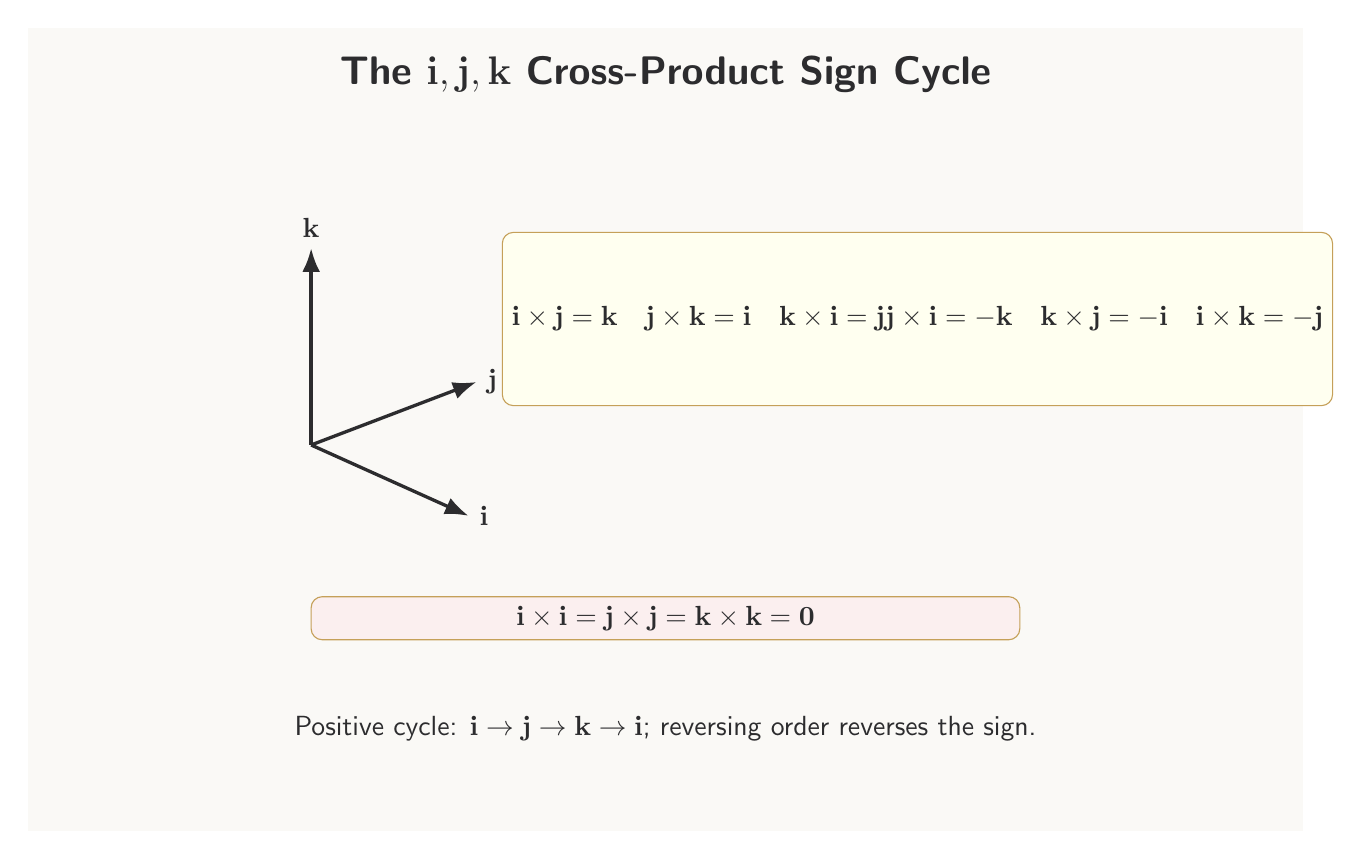
\begin{tikzpicture}[every node/.style={font=\sffamily,text=TextInk},arrow/.style={-{Latex[length=3mm]},line width=1.2pt,draw=TextInk},goldarrow/.style={-{Latex[length=3mm]},line width=1.5pt,draw=Gold}]
\fill[Canvas] (-0.6,-0.6) rectangle (15.6,9.6);

\node[font=\sffamily\bfseries\Large] at (7.5,9) {The $\mathbf{i},\mathbf{j},\mathbf{k}$ Cross-Product Sign Cycle};
\draw[arrow] (3,4.3)--(5,3.4) node[right] {$\mathbf{i}$};
\draw[arrow] (3,4.3)--(5.1,5.1) node[right] {$\mathbf{j}$};
\draw[arrow] (3,4.3)--(3,6.8) node[above] {$\mathbf{k}$};
\node[draw=Gold,fill=Ivory,rounded corners,minimum width=6.2cm,minimum height=2.2cm] at (10.7,5.9) {$\mathbf{i}\times\mathbf{j}=\mathbf{k}$\quad $\mathbf{j}\times\mathbf{k}=\mathbf{i}$\quad $\mathbf{k}\times\mathbf{i}=\mathbf{j}$\\[6pt]$\mathbf{j}\times\mathbf{i}=-\mathbf{k}$\quad $\mathbf{k}\times\mathbf{j}=-\mathbf{i}$\quad $\mathbf{i}\times\mathbf{k}=-\mathbf{j}$};
\node[draw=Gold,fill=SoftPink,rounded corners,minimum width=9cm] at (7.5,2.1) {$\mathbf{i}\times\mathbf{i}=\mathbf{j}\times\mathbf{j}=\mathbf{k}\times\mathbf{k}=\mathbf{0}$};
\node at (7.5,0.7) {Positive cycle: $\mathbf{i}\to\mathbf{j}\to\mathbf{k}\to\mathbf{i}$; reversing order reverses the sign.};

\end{tikzpicture}
\end{document}
